
\documentclass[a4paper,ngerman,12pt,bibliography=totoc,listof=totoc,numbers=noendperiod]{scrartcl}
%Startet das Dokument und regelt gleichzeitig Formatierungen wie Schriftgröße, Papierformat, Zahlenart, Sprache usw.

\title{Vorlage Praktikum Messtechnik}
\author{Julian Dietz}
\date{November 2022}
%Deklariert den Namen des Authors, sowie den Namen des Projekts

%Packages sind Erweiterungen des eigentlichen Programms und erleichtern Abläufe, Darstellungen, Formatierungen usw.
%Im Folgenden sind die Packages installiert, welche ich zum erstellen meiner Bachelorarbeit benötigt habe.

%%%%%%%%%%%%%%%%%%%%%%%%%%%%%%%%%%%%%%%%%%%%%%%%%%%%%%%%%
%%%%%%%%%%%%%%%%%%%%%%%%%%%%%%%%%%%%%%%%%%%%%%%%%%%%%%%%%

\usepackage[ngerman]{babel}
%Dient zur Rechtschreibkorrektur

\usepackage{titling}
%Hilft im Dokument auf den deklarierten Autor und Titel zuzugreifen 

\usepackage[style=numeric-comp,backend=biber,doi=false,isbn=false,maxnames=3,sorting=none]{biblatex}
\usepackage{csquotes}
\addbibresource{Referenzen.bib}
%Regelt die Erstellung des Literaturverzeichnisses sowie die Zitation im gesamten Bericht
%Greift gleichzeitig auf die Referenzen.bib genannte BibTex datei zu, in welcher die Quellen aufgeführt sind.

\usepackage{url}
%erzeugt schönere URLs (vorallem in den Quellen wichtig)

\usepackage{float}
%Hilft beim Anordnen von Bildern, Grafiken und Tabellen

\usepackage{abstract}
%ermöglicht das einfügen eines Abstract (Nicht relevant fürs Praktikum)

\usepackage{booktabs}
%ermöglicht das erstellen von schöneren Tabellen 

\usepackage{subfigure}
%lässt den Benutzer mehrere Grafiken/Bilder in einer Abbildung darstellen

\usepackage{pdfpages}
%ermöglicht das einbinden von eigenständigen PDF Dokumenten 

\usepackage{siunitx} 
\sisetup{locale = DE}
%vereinfacht den benötigten Syntax zum Benutzen von SI Einheiten und Mathematischen Gleichungen mit dem deutschen Standart

\usepackage{tikz}
%Freies Anordnen von Bildern und Text in Relation zueinander, sowie Möglichkeiten Bilder zu bearbeiten
%Verfügt auserdem über die Möglichkeit Grafiken und Diagramme in Latex zu erstellen

\usepackage[format=plain,labelfont=bf]{caption}
\captionsetup[table]{position=above}
%verschönert die Abbildungs- und Tabellenbeschriftungen. Für Tabellen werden die Beschriftungen über der Tabelle angezeigt

\usepackage{icomma}
%Für den korrekten Abstand der Kommas in Dezimalzahlen und in Gleichungen

\usepackage{amsmath}
%elementares Paket für Gleichungen. Verschönert diese und erleichtert die Benutzung von Gleichungen.

\usepackage{graphicx}
%mehr Optionen beim Einbinden und anordnen von Bildern und Grafiken

\usepackage{setspace}
%Für den richtigen Zeilenabstand

\usepackage[left=3.5cm, right=2.3cm, top=3cm, bottom=2.5cm]{geometry}
%Regelt die Seitenabstände

\usepackage[headsepline=true, markcase=noupper]{scrlayer-scrpage}
%Regelt alle Einstellung bezüglich Kopf- und Fußzeile
\pagestyle{scrheadings}
\headheight 16pt
\setcounter{secnumdepth}{3}                       
% Setzt den Zähler für die Abschnittsnumerierung auf eine Tiefe von 10. Alle Abschnitte werden nummeriert.
\setcounter{tocdepth}{3}   
% Setzt die Tiefe für das Inhaltsverzeichnis auf eine Tiefe von 10. Alle Abschnitte werden aufgeführt.
% Abschnittsnummer und Überschrift
\automark{section}
\ihead{\headmark}
\chead{}
\ohead{\pagemark}
\cfoot{}
\setlength{\parindent}{0pt}
%Einschub nach Absätzen und Zeilenumbrüchen
\renewcommand*{\headfont}{\normalfont}

\usepackage{enumitem}


%%%%%%%%%%%%%%%%%%%%%%%%%%%%%%%%%%%%%%%%%%%%%%%%%%%%%%%%%
%%%%%%%%%%%%%%%%%%%%%%%%%%%%%%%%%%%%%%%%%%%%%%%%%%%%%%%%%

\begin{document}

\thispagestyle{empty}

\begin{center}

\includegraphics[height=3.0cm]{Bilder/Deckblatt/HSU_Logo.png}   
\end{center}

\begin{center}

\vspace*{0.50cm}

\Large
\textbf{Praktikumsbericht}\\
 
\vspace*{1cm}
\huge
\textbf{TITEL DES BERICHTES}
 	
\vspace*{1.0cm}

\large
erstellt von\\

\vspace*{0.5cm}

\Large
HIER NAMEN EINFÜGEN \\

\vspace*{2cm}

\end{center}

\large
Gruppennummer: HIER GRUPPENNUMMER\\

\large 
\noindent
Versuchsnummer: HIER VERSUCHSNUMMER\\

\large
Name des Betreuers: NAME\\

\large
Datum des Versuchs: DATUM\\
 
%\vspace{4cm}

	
\begin{tikzpicture}
\node {
\includegraphics[width=\textwidth]{Bilder/Deckblatt/HSU_Swoosh.png}};
\draw (0,-3) node {Professur für Messtechnik};
\draw (0,-4) node {Helmut-Schmidt-Universität, Universität der Bundeswehr Hamburg};
\end{tikzpicture}


%include bindet andere .tex Dateien ein und hilft somit bei der Erstellung eines übersichtlichen Dokumentes

\pagenumbering{gobble}
\pagenumbering{Roman}
%Ab hier Seitenzahlen mit Römischen Ziffern

\include{01_Erklärung.tex}

\tableofcontents
%erstellt das vollautomatische Inhaltsverzeichnis

\clearpage
\pagenumbering{arabic}
%ab hier Seitenzahlen in Arabischen Zahlen

\section{Beispiel Kapitel Nummer 1}
In den folgenden Beispielkapiteln werden die wichtigsten Features von \LaTeX\:demonstriert. Diese sollen den Einstieg in das Programm Overleaf und die generelle Umgebung erleichtern. Diese Datei soll ein Grundgerüst für zukünftige Abschlussarbeiten sowie Praktikumsberichte und ähnliches darstellen. Es ist erwünscht, dass der Inhalt des Dokuments gelöscht wird, um die Formatierung zu verwenden.\\
Der folgende Text ist als Code in Kombination mit der kompilierten PDF zu lesen.\\

\subsection{Grundlagen}
Die wichtigsten Grundlagen findet man in sogenannten Cheatsheets, in welchen auf wenigen Seiten die wichtigsten Befehle von \LaTeX\:zusammengefasst sind. Ein solches Cheatsheet findet man unter:\\ \url{https://wch.github.io/latexsheet/} \\Beim Auseinandersetzen mit \LaTeX\: werden die wichtigsten Befehle schnell zu Automatismen, was die Benutzung erleichtert.\\
Im Folgenden werden die wichtigsten Grundlagen zum Einfügen von Tabellen, Grafiken und Zitationen kurz dargestellt. Auch Mathematische und Chemische Gleichungen lassen sich problemlos in \LaTeX einfügen, jedoch wird darauf nicht näher im Folgenden eingegangen, da das Vorgehen unter "Math mode" im verlinkten Cheatsheet beschrieben ist.

\pagebreak

\subsubsection{Tabellen}
Für Tabellen gibt es online verschiedene "LATEX Tabellengeneratoren", zum Beispiel:\\
\url{https://www.tablesgenerator.com/#}\\
Tabellen sehen dann wie folgt aus:

\begin{table}[H]
\begin{tabular}{|l|l|l|}
\hline
Beispiel & Test 1 & Test 2        \\ \hline
Farbe    & Grün   & Ultra-Violett \\ \hline
\end{tabular}
\caption[Beispiel Tabelle]{Beispiel Tabelle}
	\label{Tabelle 1}
\end{table}

Die Position der Tabelle (genauso Grafiken) wird über die eckigen Klammern hinter \textbackslash begin gesteuert.\\ Sowohl bei Abbildungen als auch bei Tabellen fügt man eine \textbackslash caption und ein \textbackslash label ein. Die Caption ist für das Tabellen- und Abbildungsverzeichnis, wohingegen das Label für die Referenzierung im Text ist (Beispiel: Tabelle \ref{Tabelle 1}). Falls man nun weitere Tabellen hinzufügt wird an dieser Stelle immer die entsprechende Nummer der Beispiel Tabelle auftauchen.
\pagebreak


\subsubsection{Grafiken}
Grafiken werden direkt in Overleaf hochgeladen. Man kann dann verschiedene Ordner (Oben Links) anlegen, um die Grafiken in sich zu strukturieren.

\begin{figure}[H]
 \centering
 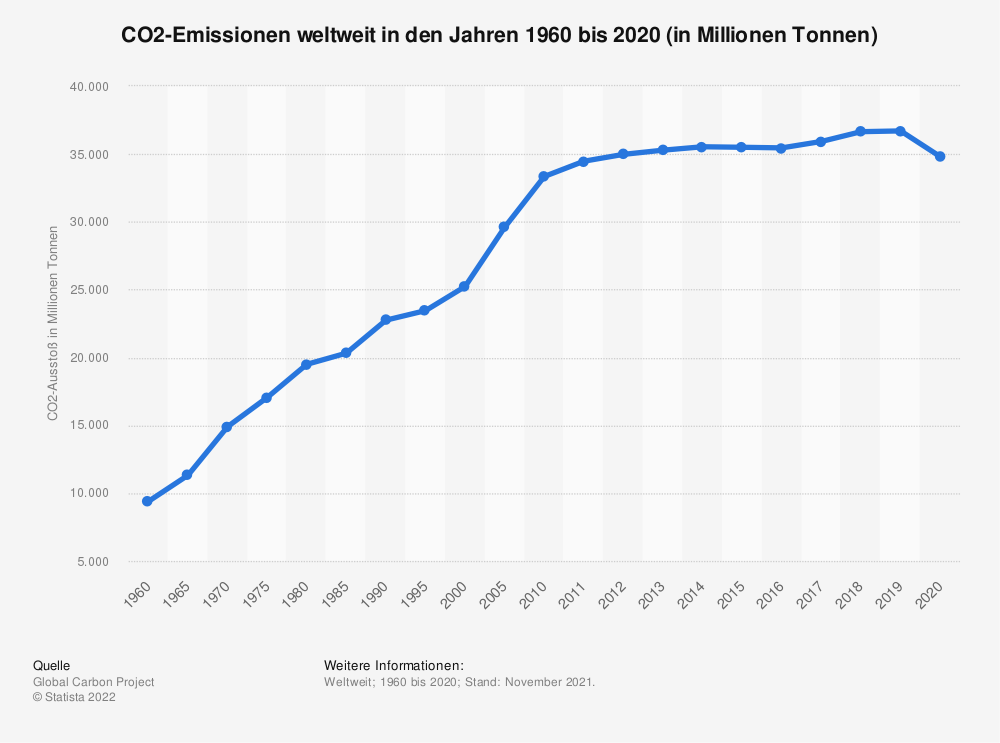
\includegraphics[width=0.8\textwidth]{Bilder/Beispiel Bilder/Klimawandel.png}
 \caption{Erschreckende Statistik zum Klimawandel}
 \label{Klimawandel}
\end{figure}
Auch hier kann  die Abbildung referenziert werden. So zeigt Abbildung \ref{Klimawandel} den weltweiten Kohlenstoffdioxid Ausstoß in Tonnen im Zeitraum von 1960 bis 2020. Die Abbildung wird auch automatisch im Abbildungsverzeichnis aufgeführt. In den eckigen Klammern können die Maße der Abbildung geändert werden.
\pagebreak
\subsubsection{Zitationen und Bibliografie}
Für die Zitationen werden in einem gesonderten Dokument alle Quellen hinterlegt. Dieses Dokument heißt hier "Referenzen.bib". In diesem Dokument können alle Arten von Quellen hinterlegt werden. Viele wissenschaftlichen Websiten bieten BIBTEX Zitationen an. Besonders hilfreich sind Literatur Generatoren wie:\\
\url{https://www.literatur-generator.de},\\
welche Zitationen zu Büchern und Artikeln für den Benutzer erzeugen können.\\
Zitationen sehen dann im Text wie folgt aus: \cite{Gates2021}. Das Aussehen der Zitationen kann bei dem benutzten Package geändert werden. Des Weiteren erstellt \LaTeX ein automatisiertes Literaturverzeichnis mit den benutzten Quellen.

\section{Beispiel Kapitel Nummer 2}
Dient nur der Veranschaulichung von Kapiteln.


\listoffigures
%erstellt das Abbildungsverzeichnis
\pagebreak

\listoftables
%erstellt das Tabellenverzeichnis
\pagebreak

\printbibliography
%erstellt das Literaturverzeichnis


\end{document}
%beendet das Dokument










